\documentclass[12pt, a4paper, openany]{report}

\usepackage[left=3cm,top=3cm, bottom=3cm, right=4cm]{geometry}

\usepackage{secdot} % Dots in Section Numbers
\usepackage[utf8]{inputenc}
\usepackage[ngerman]{babel}
\usepackage{graphicx}
\graphicspath{ {images/} }

\usepackage{fancyhdr}
\usepackage{todonotes}
\usepackage{hyperref}

\usepackage{titlesec}
\titleformat{\chapter}[hang]{\Huge\bfseries}{}{0pt}{\Huge\bfseries}
\newcommand\frontmatter{ \cleardoublepage \pagenumbering{roman}}
\newcommand\mainmatter{ \cleardoublepage \pagenumbering{arabic}}
\newcommand\backmatter{ \if@openright \cleardoublepage \else \clearpage \fi }

\usepackage[autostyle]{csquotes}
\usepackage[
    backend=biber,
    style=alphabetic,
    sortlocale=de_DE,
    natbib=true,
    url=false,
    doi=true,
    eprint=false
    ]{biblatex}
\addbibresource{literatur.bib}

\usepackage{xparse}
\DeclareDocumentCommand \footATCite{ O{} o m } {%
  \IfNoValueTF {#2} {\footnote{#1 \citeauthor{#3}, \emph{\citefield{#3}{shorttitle}}.}}
                    {\footnote{#1 \citeauthor{#3}, \emph{\citefield{#3}{shorttitle}}, S. #2}}
  }

\makeatletter
\def\mycmd{\@ifnextchar[{\@with}{\@without}}
\def\@with[#1]#2{hello #1, have you met #2?}
\def\@without#1{goodbye #1}
\makeatother

\pagestyle{fancy}
\fancyhf{}
\lhead{Jan van Dick}
\chead{\glqq Zweite Natur und Befreiung\grqq}
\rhead{\thepage}

\title{
    {Zweite Natur und Befreiung - zwischen Affirmation und Kritik}\\
    {\large Goethe Universität Frankfurt am Main}\\
    {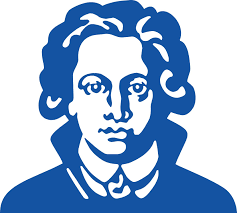
\includegraphics{logo.png}}
}
\author{Jan van Dick}
\date{\today}

\begin{document}

\maketitle
\frontmatter


\chapter*{Abstrakt}
Friedrich Nietzsches These vom Tode Gottes, dass \glqq wir\grqq{} ihn getötet haben, ist mehr als bloße Negativität. 
Müsste der Mensch nicht selbst Gott werden, um ihn getötet zu haben?.\footfullcite[Vgl.][481]{nietzsche_morgenrote_1999} 
Und der Mensch ist Gott dadurch geworden, dass er ihn \textit{geschaffen} hat, dadurch nur konnte er ihn töten. 
In dem Tod Gottes, liegt, dass Gott selbst vom Menschen gesetzt, dass er Schein ist, der sich gegen ihn verselbstständigte.
Gott ist somit geistiges Produkt des Menschen, in dem der Geist selbst wieder zur Natur sich verkehrte.
Der Tod Gottes ist die Befreiung daraus.
Der \glqq Tolle Mensch\grqq{} erklärt aber zugleich, dass nur die wenigsten von dieser Tat wissen. 
Für die Einen ist der Tod Gottes, eine untergegangene Sonne, die Befreiung also wieder eine In-Natur-Verkehrtheit.
Nur für uns \glqq geborene Räthselrather\grqq, die den Tod Gottes im vollen Umfang begreifen, ist er ein \glqq neues offenes Meer\grqq\footATCite[][573]{nietzsche_morgenrote_1999}.
Ist nun der Tod Gottes, die Befreiung aus der von ihm gesetzten Natur, das unbekannte, neue, offene, noch nie so offen gewesene Meer, oder ist er der Beginn des Wieder-in-Natur-Verkehrt-Seins, wie Christoph Menke es in der Analyse Hegels Begriffs der zweiten Natur beschreibt?\footfullcite[Vgl.][144]{menke_autonomie_2018}\\
Befreiung steht also zwischen Kritik (wieder-in-Natur-Verkehrtheit) und Affirmation (Einheit von Setzen und Sein).
Während Menke (und Hegel) Befreiung aus der zweiten Natur, nicht ohne eine neu hervorgebrachte zweite Natur, in welcher der Geist wieder in Natur verfällt lesen, erörterte ich die Frage, ob es in dem Motiv des \glqq neuen offenen Meeres\grqq{} und der \glqq geborenen Räthselrather\grqq{} bei Nietzsche, eine Befreiung aus der fortwährenden In-Natur-Verkehrtheit geben kann.
Es ist die Frage nach einer dritten Befreiung neben der Befreiung aus der 1. und der 2. Natur. 
Die Antwort dazu wird sich in der Arbeit als Ergebnis des Unterschiedes der \glqq Erkennenden\grqq{} bei Nietzsche geben:
Zwar kann Befreiung aus der Natur nicht ohne Setzen einer zweiten Natur geschehen, aber die Befreiung, die sich in dem Bewusstsein ihrer eigenen Kritik vollzieht, ist zugleich über ihrer eigene Befreiung hinaus.
Die dritte Befreiung ist damit allerdings keine Befreiung aus der Befreiung.
Befreiung bleibt notwendig: der Mensch kann Freiheit nicht \textit{haben}, er muss sie immer wieder selbst hervorbringen.


\tableofcontents

\mainmatter

\chapter{Einleitung}
So, wie Friedrich Nietzsche in dem Aphorismus vom \glqq Tollen Menschen\grqq{} in \textit{Die fröhliche Wissenschaft} die These vom Tode Gottes entfaltet, enthält sie weit mehr als die bloße Negation Gottes;
in ihr steckt eine dialektische Konzeption der Begriffe (zweite) Natur und Befreiung.\footfullcite[Vgl.][481]{nietzsche_morgenrote_1999}
Diese beiden Begriffe möchte ich aus der sprachgewaltigen und metaphergeladenen Sicht Nietzsches, sowie der von Christoph Menke rekonstruierten Perspektive Hegels untersuchen.
Beide Begriffe entfalten sich in ihrem Doppelcharakter: zweite Natur - Kritik und Affirmation, Befreiung - Macht und Ohnmacht des Geistes.
In der zweiten Natur schlägt Setzen in Sein um; hierin liegt zum Einen die Verwirklichung des Geistes (Affirmation), zum Anderen, die In-Natur-Verkehrtheit, der Tod des Geistes im Geist (Kritik).\footfullcite[Vgl.][145]{menke_autonomie_2018}
Ebenso verhält es sich mit dem Begriff der Befreiung: 
Sie ist 1. die \textit{Macht} des Geistes neues Hervorzubringen und die scheinbare Notwendigkeit des Bestehenden zu durchbrechen, 
2. aber die \textit{Ohnmacht} des Geistes, da die Befreiung nie abgeschlossen ist; die Macht der Befreiung ist die Schaffung einer \glqq neuen\grqq{} zweiten Natur, aus der der Geist sich befreite und nun erneut befreien muss.\footATCite[Vgl.][80]{menke_autonomie_2018}\\
Doch während in Hegels Deutung der Geist in der Befreiung aus der zweiten Natur, auf Grund der Endlichkeit des menschlichen Geistes, wieder in Natur verfällt, scheint bei Nietzsche in der Metapher des neuen, offenen Meeres, die Perspektive die ewige Wiederholung der In-Natur-Verkehrtheit zu überwinden, gegeben zu sein.
Zugleich betonen sowohl Hegel, als auch Nietzsche Freiheit als nicht-gegeben: 
Freiheit wird bei beiden so gedacht, dass man sie \glqq nicht nur hat, sondern auch beständig  noch erwirbt und erwerben muss\grqq\footATCite[][637]{nietzsche_morgenrote_1999}. 
Freiheit ist die Befreiung aus der jeweiligen Unfreiheit.\footfullcite[Vgl][227]{adorno_negative_dialektik_2003} \\
Die Dialektik zwischen Freiheit und Notwendigkeit, Geist und Mechanismus, Endlichkeit und Unendlichkeit des Geistes, ist demnach Grundlage meiner Arbeit. 
Die Leitfrage der Arbeit also: \textit{gibt es in Nietzsches Philosophie eine Möglichkeit der Überwindung der Notwendig-in-Natur-Verkehrtheit des Geistes?}\\
Aus der Position des oben erwähnten \glqq Tollen Menschen\grqq{} liegt es nahe, diese Möglichkeit in dem \textit{Vollzug} der Befreiung zu denken. 
Genauer: in einer Form des Bewusstseins in der Tätigkeit der Befreiung; 
eine Befreiung, die sich im Bewusstsein ihrer eigenen Kritik vollzieht.
Zu Fragen ist, ob dieses Bewusst-Werden eine Arbeit des einzelnen Individuums ist, oder ob es aus der Struktur des Allgemeinen, aus der zweiten Natur selbst, hervorgehen kann.\\

Der Begriff der zweiten Natur soll zunächst aus der Position Hegels heraus entwickelt werden, als eine Kritik an Kants Begriff der Autonomie. 
Darin ergibt sich, wie oben angegeben, die Grenze des von Menke erarbeiteten Begriffs der Befreiung:
Macht und Ohnmacht der Befreiung: Freiheit und Unfreiheit bleiben untrennbar miteinander verbunden.
Durch die Hinzunahme Nietzsches, soll versucht werden über diese Grenze hinauszugehen.
Dazu soll zunächst der Begriff der zweiten Natur aus der Perspektive Hegels erläutert werden. 
In einem \hyperref[abschnitt_1]{ersten Schritt} soll demnach der Hegelsche Begriff der zweiten Natur anhand von folgendem Zitat Menkes rekonstruiert werden:
\begin{itemize}
    \item[] Die Gewohnheit als zweite Natur [ist] geistig oder frei [...], insofern sie ein Ausdruck des Wollens (oder ein Setzen) ist, und [...] mechanisch oder unfrei [...], weil sie, einmal gesetzt, selbstständig und unbewusst wirkend ist.\footATCite[][145]{menke_autonomie_2018}
\end{itemize}
Die Struktur des ersten Teils ergibt sich aus den zu klärenden Begriffen. 
Zuerst soll der Begriff der Gewohnheit aus der Sittlichkeit, als Schritt über den \glqq bloß moralischen Standpunkt[]\grqq\footfullcite[][§ 135, S.139]{hegel_grundlinien_2017} hinaus, erläutert werden (a). 
Daraus ergibt sich der Begriff des \glqq geistigen Mechanismus\grqq, in welchem die Gewohnheit sich als \glqq geistig oder frei\grqq{} und \glqq mechanisch oder unfrei\grqq{} ergibt.\footATCite[][145]{menke_autonomie_2018} (b).
Schließlich soll der Begriff der zweiten Natur aus Hegels Perspektive, seinen Abschluss finden in der Dialektik zwischen endlichem und unendlichem Geist und dem Doppelcharakter der zweiten Natur als Kritik und Affirmation (c).\\
In einem \hyperref[abschnitt_2]{zweiten Schritt} soll gezeigt werden, dass bei Nietzsche ein ähnlicher Begriff der zweiten Natur aufgezeigt werden kann.\footnote{Ich halte diesen Schritt unter anderem des deshalb für sinnvoll, weil er rechtfertigt, warum ich meine, mit Nietzsche überhaupt über Menkes Begriff der Befreiung hinausgehen zu können.}
Dabei soll bereits auf die Beantwortung der Leitfrage vorbereitet werden.
Zunächst soll der Begriff der zweiten Natur anhand von Nietzsches Begriff des \textit{Scheins} erläutert werden (a).
Die Befreiung aus dem (sog.) Schein wird darauffolgend in der Unterscheidung des Schauspielers und der Rolle aufgegriffen (b). 
Abschließend sollen beide Begriffe nochmals in dem Absatz über den tollen Menschen analysiert und zusammengebracht werden (c).
In der Darlegung Nietzsches Position wird der Begriff \glqq Bewusstsein der Scheinhaftigkeit\grqq{} bereits eine wichtige Rolle einnehmen und dient der späteren Beantwortung der Leitfrage.\\
Im \hyperref[abschnitt_3]{dritten Abschnitt} soll die Befreiung aus der zweiten Natur erläutert werden, da diese, im Vergleich zur Befreiung aus der ersten Natur bei Hegel und Menke und letztendlich auch bei Nietzsche, uneindeutig bleibt.
Wie Befreiung aus der zweiten Natur überhaupt möglich ist und wie diese sich konkret vollzieht, ist notwendig, um zu diskutieren wie über diese hinausgegangen werden kann.\\
Im vierten und \hyperref[abschnitt_4]{letzten Schritt} soll es abschließend zu einer Diskussion und Beantwortung der Leitfrage kommen. 


\chapter{Hauptteil}
Die folgende Diskussion um Befreiung und zweite Natur wird ihren Ausgangspunkt in der Kritik der Autonomie finden, aus dem ich zu Hegels Begriff der Sittlichkeit kommen werde. 
Es mag merkwürdig anmuten, dass ich gerade mit der Kritik an der Autonomie beginne und hier, als Ausgangspunkt dieser Kritik, den Begriff einer positiven Bestimmung der Freiheit hinterfrage,
wo die Leitfrage meiner Arbeit doch letztendlich auf einen positiven Begriff der Freiheit hinausläuft, auf eine Befreiung, die die Unfreiheit hinter sich lassen kann.
Dennoch und trotzdem, liegt meiner Arbeit, wie den beiden Autoren, zu jeder Zeit Adornos Bestimmung der Freiheit als Befreiung aus der jeweiligen Unfreiheit zu Grunde.
Der Versuch eines Hinausgehen, über den Begriff der Befreiung hinaus oder durch ihn hindurch, hin zu einem positiven Begriff von Freiheit, ist ohne die Kritik an dem positiven Begriff der Freiheit, zum Scheitern verurteilt.
Meine Vorstellung eines positiv bestimmten Freiheitsbegriffs, oder die Befreiung über die Befreiung hinaus, ist die Befreiung, die sich als Unfreiheit weiß; die Befreiung also, die weder positiv noch negativ, sondern beides ist.

\section{Zweite Natur bei Hegel}\label{abschnitt_1}
Freiheit so zu verstehen, dass man sie beständig noch erwerben muss\footATCite[Vgl.][636]{nietzsche_morgenrote_1999}, bedeutet Freiheit als Befreiung zu verstehen. 
Freiheit also als einen Akt zu verstehen, der noch, oder immer wieder geschehen muss.
Damit heißt Freiheit als Befreiung zu denken, wie Hegel, Menke, Adorno und, wie ich argumentieren werden, auch Nietzsche, es tun,  Freiheit negative zu verstehen und aus der Negation heraus zu begreifen.
Immanuel Kant versucht in der Bestimmung der Freiheit als Selbstgesetzgebung, Freiheit so zu bestimmen, dass dieser Akt der Negation verschwindet. 
Dieser Versuche ist bei Kant zugleich der Versuch das Paradox der Autonomie aufzulösen. 
Hegels Kritik der Autonomie, versucht hingegen aufzuzeigen, dass sich dieses Paradox in der Selbstgesetzgebung auch bei Kant erneut wiederholt.
Ich möchte zunächst anhand von Hegels Kritik der Autonomie den Begriff der Sittlichkeit erarbeiten.
Aus diese komme ich zur Gewohnheit, welche
\begin{itemize}
    \item[] [...] als zweite Natur geistig oder frei ist, insofern sie ein Ausdruck des Wollens (oder ein Setzen) ist, und mechanisch oder unfrei ist, weil sie, einmal gesetzt, selbstständig und unbewusst wirkend ist.\footATCite[][145]{menke_autonomie_2018}
\end{itemize}
Hieran zeigt sich, dass in der Sittlichkeit das Paradox der Autonomie erneut auftritt. 
Anhand des Zitates, werde ich die sich hier entfaltende Dialektik von Geist und Mechanismus, sowie Kritik und Affirmation beschreiben und daraus die Begriffe zweite Natur und Befreiung erarbeiten und an ihnen den Ausweg aus dem Paradox skizzieren.

\subsection{(a) Autonomie und Sittlichkeit}

Autonomie bedeutet zunächst Gesetz und Freiheit nicht als einander gegenübergestellt, sondern als sich gegenseitig ergänzend und bestimmend zu betrachten: 
Nicht in dem blinden Folgen meiner sinnlichen Triebe, sondern in dem Handeln nach dem Gesetzt bin ich frei. 
Und ein Gesetzt ist nur dasjenige, unter dessen Befolgung ich frei bin. 
Autonom zu sein bedeutet also meinem selbst gegebenem Gesetzt zu folgen. 
Autonomie bedeutet, dass freies Wollen und verpflichtendes Sollen in eins fallen.\footATCite[Vgl.][19]{menke_autonomie_2018}


\subsection{(b) Dialektik von Geist und Mechanismus}
\subsection{(c) Dialektik von Kritik und Affirmation}
\section{Zweite Natur bei Nietzsche}\label{abschnitt_2}
\subsection{(a) Was bedeutet Schein?}
\subsection{(b) Der Schauspieler und die Rolle}
\subsection{Exkurs: Nietzsche - Natur und Antisemitismus}
In dem vorherigen Abschnitt stellt Nietzsche den Schauspieler und die Rolle gegenüber. 
In dieser Gegenüberstellung tritt noch eine dritte \glqq Persönlichkeit\grqq{} auf: der Baummeister. 
Außerdem identifiziert Nietzsche den Schauspieler mit den Juden und den Frauen. 
Diese Gegenüberstellungen und Identifizierungen möchte ich zum Anlass nehmen auf einen weiteren Punkt einzugehen, der mit den Gegenstand der Arbeit nicht Unmittelbar, aber Mittelbar zusammenhängt. 
Für Nietzsche ist, wie Eingangs beschrieben, Schein nicht der Gegensatz zu dem Wesen, zur Natur, sondern Schein, oder Kunst, ist das Wirkende und Lebende selber.\footATCite[Vgl.][416]{nietzsche_morgenrote_1999} 
Diese Stelle, und andere vorher erwähnte Stellen, legen nahe, dass es für Nietzsche überhaupt gar nicht etwas, wie (erste) Natur gibt, sondern, dass alles Schein, zweite, vom Menschen geschaffene Natur ist.
Wie verhält sich dies allerdings zu dem Baumeister, der sich durch Kraft und Mut auszeichnet, die Gesellschaft zu bauen, für die \glqq wir\grqq{} nicht mehr das richtige Material sind etc. 
Der im Gegensatz zu dem Schauspieler, dem Künstler, dem Wechselhaften, Ungebundenen, Heimatlosen steht, der \glqq natürlich\grqq{} und \glqq von Natur aus\grqq{} so ist.\\
Diese Gegenüberstellung erscheint bei Nietzsche zunächst, als Antisemitismus. 
Dem Schauspieler, den Frauen, den Juden wird der Baummeister, der ehrliche, mutige, beinahe mag man sagen \glqq deutsche\grqq{} Wesenszug entgegengestellt.
Das wir alle schon zu sehr Schauspieler geworden seinen, zu sehr amerikanisiert seien, wie Nietzsche schreibt, wirkt wie die völkische, oder zumindest konservative  Kritik an der jüdischen, wahlweise liberalen oder bolschewikischen Verschwörung.
Auf ähnliche Weise könnten hier Nietzsches Beschäftigungen mit dem \glqq Sklavenaufstand der Moral\grqq{} herangezogen werden, in welchen Nietzsche die Schwachen dafür kritisiert aus einem Gefühl der Unterlegenheit heraus den Starken ihre Moral aufzuzwingen. 
Die Sklavenmoral steht bei Nietzsche im schroffen Gegensatz zu der Moral \glqq alle[r] vornehme[n] Moral[, die] aus einem triumphierenden Ja zu sich selbst herauswächst\grqq\footfullcite[][S. 10?]{nietzsche_jenseits_2014} 
An dieser Stelle wird jedoch ersichtlich, dass Nietzsche Identifikation des Schauspielers mit den Juden und Frauen gerade aus der Entgegengesetzten Richtung stammt:
die Scheinbare Kritik an den Juden, sie sein \glqq jenes Volk der Anpassungskunst par excellence\grqq\footATCite[][609]{nietzsche_morgenrote_1999} mutet antisemitische, muss aber aus dem selben Blickwinkel gedeutet werden, aus dem heraus Nietzsche die Sklavenmoral kritisiert:
dann wird deutlich, dass Nietzsches Kritik sich nicht gegen die Juden wendet, sondern viel gegen die, die aus einem Gefühl der eigenen Unterlegenheit die Macht der Juden aus der Perspektive der Sklavenmoral heraus kritisieren. 
Anders gesagt: aus der Perspektive Nietzsches Kritik am Ressentiment, gehören nicht die Juden und die Frauen und die Schauspieler zum Ressentiment, sondern gerade die Antisemiten, die Gender-Kritiker, die Baumeister. 
Auch an den Stellen also, an den Nietzsche scheinbar das Natürliche, Angeborene, hervorhebt, zeigt sich, dass sich dieses eben nur durch das \glqq Ja-sagen zu sich selber\grqq{} durch das Sich-selbst-Hervorbringen, das Spielen und mit der eigenen \glqq Natur\grqq{} entwickelt, dass nur diejenigen Vornehm sind, die ihre scheinbare Natur bespielen und wieder in Kunst aufgehen lassen.

\subsection{(c) Gott ist tot!}
\section{Was heißt Befreiung aus der zweiten Natur}\label{abschnitt_3}
\section{Das offene Meer?}\label{abschnitt_4}

\chapter{Fazit}

\backmatter

\printbibliography
 
\end{document}
